In this chapter, we will delve into the conposition of our dataset and perform exploratory analysis on the dataset.

\section{Dataset Exploration}

In our research we were utilising T2-weighted MRI images to help with segmentation tasks. T2-weighted images are a specific genre of MRI scans manifested by the heightened intensity in fluid-rich structures, while their fat-laden counterparts appear darker.

In enriching the diversity of our dataset, we have judiciously incorporated three variants of MR images. Each class of image contains 233 MR scans, which are obtained by radiologists in St. Mark's Hospital.

A summary describing the unique features and applications of each variant is as follows, and the difference between images can be further visualised in \autoref{fig:mri} below.

\begin{itemize}
    \item \textbf{Axial T2-weighted Images}: Projected along the axial plane, these images provide a top-down representation of anatomical structures and are especially beneficial in examining anatomical correlations.
    \item \textbf{Coronal T2-weighted Images}: Imaged along the coronal plane, these scans offer a frontal perspective of the anatomy. These images are reputable for their proficient highlighting of fluid-filled structures and lesions.
    \item \textbf{Post-Contrast Axial T2 Images}: These images are captured after administering a contrast agent and enhance tissue contrast, thereby providing enriched insights into the nature of lesions.
\end{itemize}

\begin{figure}[htp]
    \centering
    \begin{subfigure}[b]{0.32\textwidth}
        \centering
        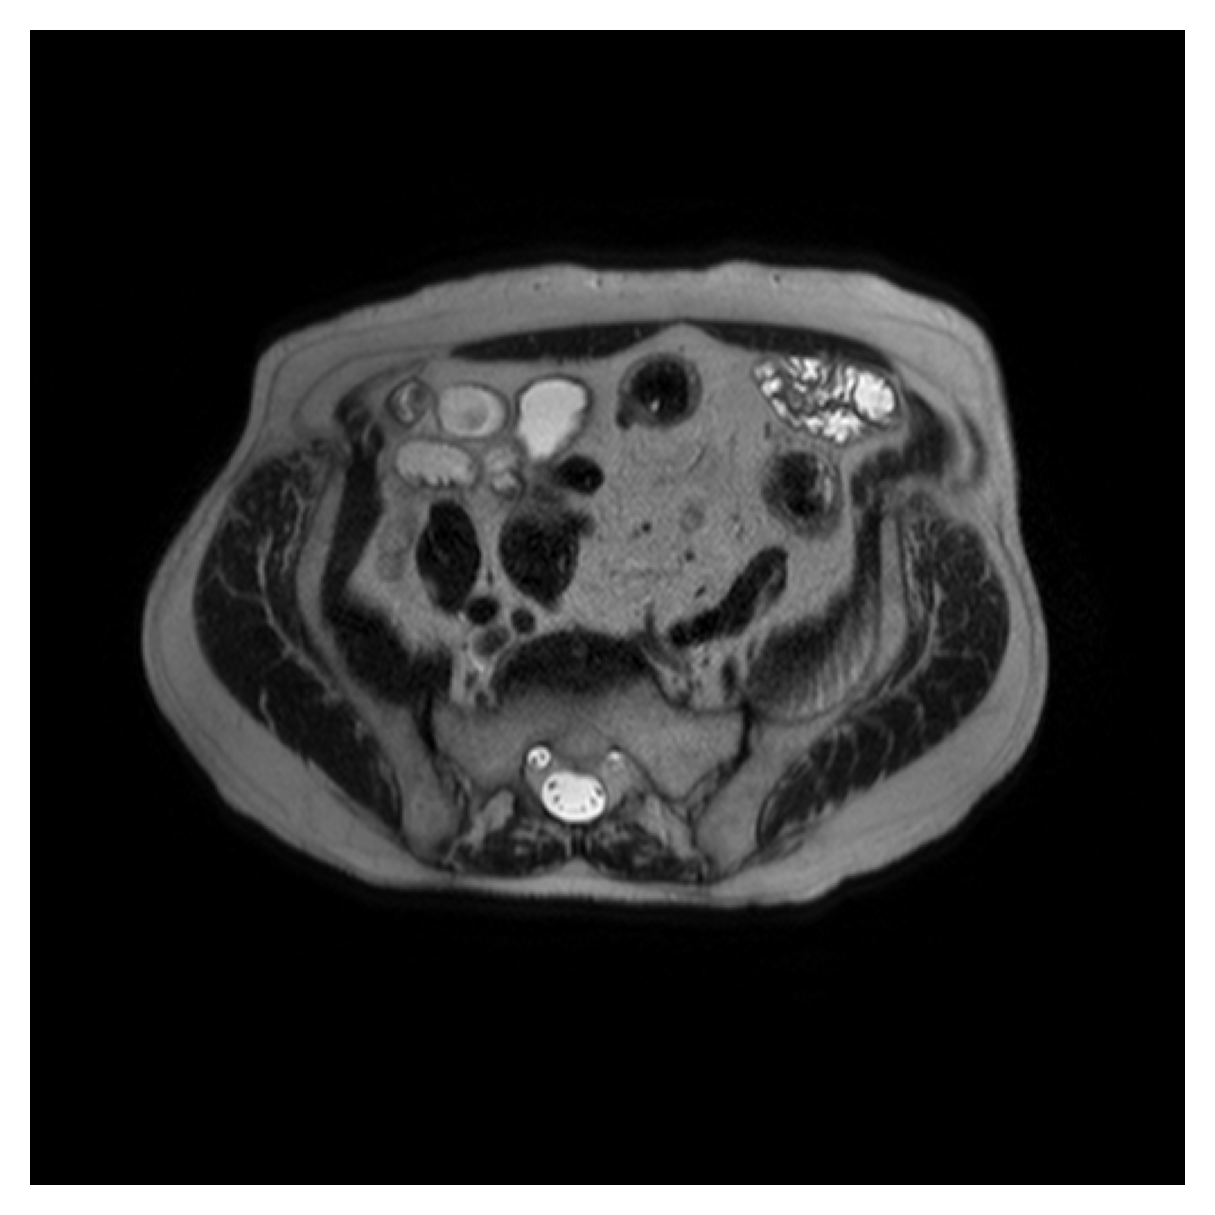
\includegraphics[width=\textwidth]{./figures/axial.png}
        \caption{Axial}
        \label{fig:axial}
    \end{subfigure}
    \hfill
    \begin{subfigure}[b]{0.32\textwidth}
        \centering
        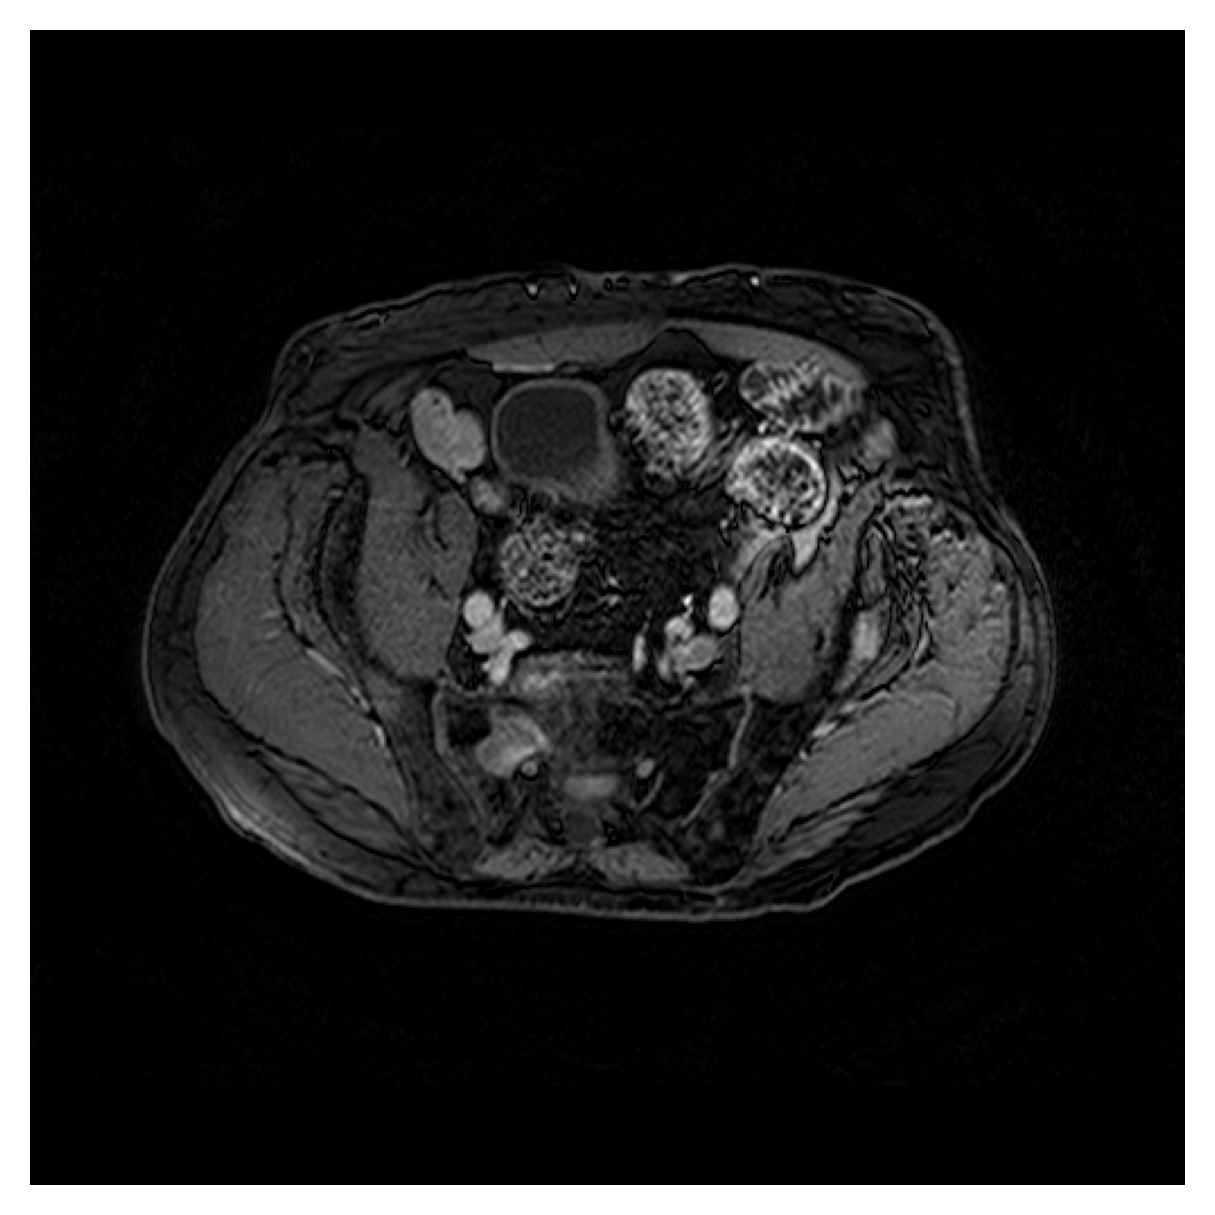
\includegraphics[width=\textwidth]{./figures/axial_postcon.png}
        \caption{Post-Contrast Axial}
        \label{fig:axial-postcon}
    \end{subfigure}
    \hfill
    \begin{subfigure}[b]{0.32\textwidth}
        \centering
        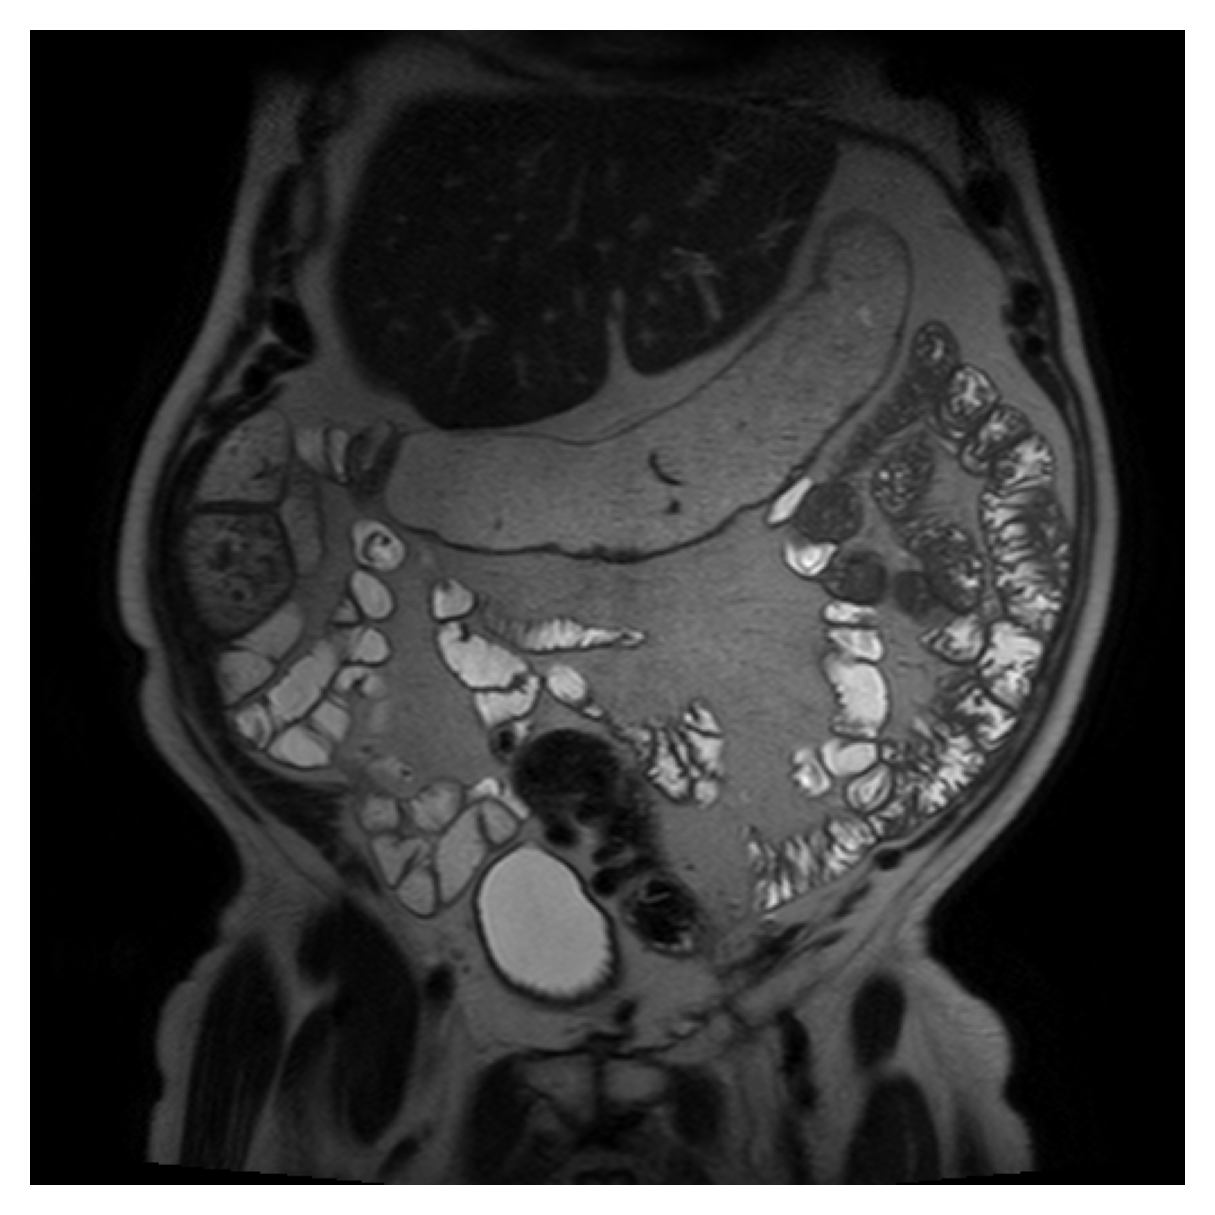
\includegraphics[width=\textwidth]{./figures/coronal.png}
        \caption{Coronal}
        \label{fig:coronal}
    \end{subfigure}
    \caption{T2-Weighted MRI with different modalities in the dataset}
    \label{fig:mri}
\end{figure}

The strategic incorporation of three distinct forms of MR images enriches our dataset, transforming it into a comprehensive repository designed to master the intricate task of segmentation. However, it is still obvious to see potential obstacles such as MRI artefacts originating from patient movement or the overarching issue of data scarcity posing challenges to the success of the segmentation task

The limited availability of annotated data not only affects the trajectory of the model training but also curtails our ability to effectively evaluate the model performance due to the restricted availability of testing data.

However, this scarcity of data that fuels our quest for alternative annotated datasets to augment model training. The following chapter provides a detailed discussion of our innovative approach to addressing this challenge.

\section{Dataset Specification}

To have a detailed peek for the composition of our dataset, for each type of Image, our dataset includes 113 abnormal cases and 120 normal cases in terms of diseased tissue in the abdominal scan. In addition to images, we also have a collection of centerline coordinates representing the colon in the MR image, although these are not available for every image. Furthermore, a select set of human-annotated ground truth results is included.

The generation of colon centerline coordinates is a meticulous process, performed by radiologists via manual slice-by-slice inspection. Following their careful examination, they annotate the relevant slices with reference points linked to the colon. These annotations are archived as compressed XML files, colloquially referred to as \textbf{traces files}.

This storage format serves a dual purpose. Firstly, it facilitates visual inspection and analysis within the framework of medical imaging by clinical experts. Secondly, it empowers developers to navigate through the XML tree to gather valuable information about the centerline coordinates. It is worth noting that the preliminary 20\% of the points are often deemed the most accurate, typically representing the interval in which the terminal ileum is situated.

Upon closer examination, the centerline and ground truth annotation distribution is shown in \autoref{table:dataset}.

\begin{table}[htp]
    \centering
    \begin{tabular}{|c|c|c|c|}
    \hline
    Modality & Total Centerlines & \begin{tabular}[c]{@{}c@{}}Centerlines\\ (abnormal:normal)\end{tabular} & \begin{tabular}[c]{@{}c@{}}Ground Truth\\ (abnormal:normal)\end{tabular} \\
    \hline
    Axial & 103 & 59:44 & 18:20 \\
    \hline
    Coronal & 93 & 46:47 & 18:30 \\
    \hline
    Post-Contrast & - & - & 13:20 \\
    \hline
    \end{tabular}
    \caption{Distribution of centerlines and ground truth segmentations for different MR images}
    \label{table:dataset}
    \end{table}

Our diverse and comprehensive dataset provides thoughtful insights for analysis and a solid foundation for reliable model training.

\section{Ground Truth Segmentations}

The ground truth segmentations delivered by our panel of clinical experts are assigned with varying semantic meanings, each corresponding to unique label IDs. The specifics of these relationships are highlighted in Table \ref{tab:segmentation-label-id}. To gain a clear overview of the segmentation, I drew ten samples from each type of labelled image data and investigate the label distribution. It is thereby graphically demonstrated in \autoref{fig:label-distribution} represented on a logarithmic scale.

\begin{figure}[htp]
    \centering
    \begin{subtable}[htp]{0.48\textwidth}
        \centering
        \begin{tabular}{|c|c|}
            \hline
            Label & ID \\
            \hline
            Background & 0 \\
            \hline
            Abnormal T.I. & 1 \\
            \hline
            Normal T.I. & 2 \\
            \hline
            Colon & 3 \\
            \hline
            Colon & 4 \\
            \hline
            Appendix & 6 \\
            \hline 
        \end{tabular}
        \caption{Label-ID representations used across manual segmentations}
        \label{tab:segmentation-label-id}
    \end{subtable}
    \hfill
    \begin{subfigure}[htp]{0.5\textwidth}
        \centering
        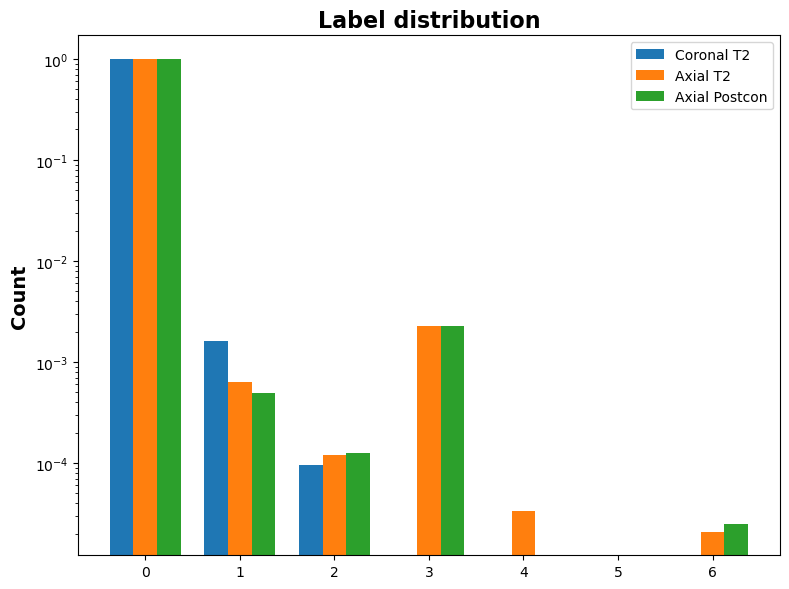
\includegraphics[width=\textwidth]{./figures/label_distribution.png}
        \caption{Illustration of Segmentation Label Distribution}
        \label{fig:label-distribution}
    \end{subfigure}
       \caption{Detailed breakdown of segmentation specifics and label distribution across diverse categories of image data}
       \label{fig:manual-segmentation}
\end{figure}

From the results, a salient observation is the predominance of the background label in the voxel classes of the ground truth segmentation results. Its pronounced presence approximates to one, rendering other voxel labels relatively insignificant and emphasizing the challenges intrinsic to abdominal MRI segmentation.

This raised a need for us to rethink the segmentation scope. Given the relative insignificance of portions other than the background, the informational value they contribute toward the training process is marginal at best. This limited contribution not only impedes the ability of model to classify effectively within these regions but increases the risk of false-positive classifications considering the comparison between the remaining regions versus the background. However, to alleviate this issue, we simplify the scenario into a binary classification problem, interpreting all non-background voxels as general T.I. regions. Accurate segmentation of this region holds significant implications for enabling clinical experts to diagnose Crohn's disease at an early stage.

This insight has inspired us to consider utilizing the centerline coordinates as a guiding factor for future initiatives. Specifically, we are contemplating two potential applications: augmenting the data through bounding box applications or minimizing the search space by cropping the image. This could balance the label distribution between background and T.I. regions, thereby improving the suitability of the segmented images for subsequent analyses. Ultimately, these initiatives aim to overcome the challenges identified in our exploration of ground truth segmentations.


